\documentclass{beamer}

\usepackage[utf8x]{inputenc}
\usepackage{graphicx}
\usepackage{amsthm,amssymb,amsbsy,amsmath,amsfonts,amssymb,amscd}
\usepackage{dsfont}
\usepackage{array}
\newcolumntype{N}{@{}m{2pt}@{}}
\useoutertheme[subsection=false]{miniframes}
\usepackage{lmodern}

\setbeamercolor{author in head/foot}{fg=gray,bg=white}
\setbeamercolor{title in head/foot}{fg=gray,bg=white}
\setbeamercolor{page number in head/foot}{fg=gray,bg=white}
\setbeamercolor{section in head/foot}{bg=black,fg=gray}
\setbeamercolor{subsection in head/foot}{bg=black,fg=gray}

%%%%%%%%%%%%%%%%%%%%%%%%
% GENERAL BEAMER STYLE :

\setbeamertemplate{footline}{
  \hbox{%
    \begin{beamercolorbox}[wd=.2\paperwidth,ht=2ex,dp=1ex,left]{author in head/foot}%
      \hskip1em\usebeamerfont{author in head/foot}\insertshortauthor
    \end{beamercolorbox}%
    \begin{beamercolorbox}[wd=.7\paperwidth,ht=2ex,dp=1ex,center]{title in head/foot}%
      \usebeamerfont{title in head/foot}\insertshorttitle
    \end{beamercolorbox}%
    \begin{beamercolorbox}[wd=.1\paperwidth,ht=2ex,dp=1ex,right]{page number in head/foot}%
      \usebeamerfont{page number in head/foot}\insertframenumber{} / \inserttotalframenumber
      \kern1em 
    \end{beamercolorbox}
  }
}

\setbeamercolor{alerted text}{fg=red!80!black}
\setbeamercolor{itemize/enumerate subbody}{fg=gray!70!black}
\setbeamertemplate{itemize item}[square]
\setbeamertemplate{itemize subitem}[triangle]%{{\textendash}}
\setbeamerfont{itemize/enumerate subbody}{size=\footnotesize}
\setbeamerfont{itemize/enumerate subitem}{size=\footnotesize}

\setbeamertemplate{navigation symbols}{}

\AtBeginSection{
\begin{frame}
    \begin{centering}
    \begin{beamercolorbox}[sep=12pt,center]{part title}
    \usebeamerfont{section title}\insertsection\par
    \end{beamercolorbox}
    \end{centering}
\end{frame}
}

 

%\title[Short course on Statistical Modelling for Optimization -- lecture 1/4]{ \small Short course Statistical Modelling for Optimization -- lecture 1/4 \\ \vspace{3mm} \LARGE Statistical models in engineering}
%\institute[Mines St-\'Etienne]{Nicolas Durrande (durrande@emse.fr) \\ Jean-Charles Croix (jean-charles.croix@emse.fr) \\ Mines St-\'Etienne -- France}
%\author[Pereira, June 2017]{June 2017 -- Universidad Tecnol\'ogica de Pereira -- Colombia}
\title[\'Ecole chercheurs MEXICO]{ \small \'Ecole chercheurs MEXICO, La Rochelle, Mars 2018\\ \vspace{3mm} \LARGE Introduction to statistical modelling}
\author[La Rochelle, March 2018]{Nicolas Durrande, nicolas@prowler.io}
\institute[]{PROWLER.io, Cambridge (UK) -- Mines St-\'Etienne (France)}
\date{\null}

\DeclareMathOperator*{\Var}{var}
\DeclareMathOperator*{\E}{E}
\DeclareMathOperator*{\Cov}{cov}
\newcommand\PR[1]{\mathrm{P}\left(#1 \right)}
\newcommand\PS[1]{{\langle #1 \rangle}_\mathcal{H}}
\newcommand\PSi[2]{{ \left \langle #1 \right \rangle}_{\! #2}}
\newcommand\N[1]{{|| #1 ||}_\mathcal{H}}
\newcommand\Ni[2]{{|| #1 ||}_{\! #2}}
\newcommand\dx{\, \mathrm{d}}
\newcommand\textequal{\rule[.4ex]{4pt}{0.4pt}\llap{\rule[.7ex]{4pt}{0.4pt}}}
\newcommand{\argmin}{\operatornamewithlimits{argmin}}
\makeatletter
\newcommand{\shorteq}{%
  \settowidth{\@tempdima}{a}% Width of hyphen
  \resizebox{\@tempdima}{\height}{=}%
}
\makeatother

%%%%%%%%%%%%%%%%%%%%%%%%%%%%%%%%%%%%%%%%%%%%%%%%%%%%%%
%%%%%%%%%%%%%%%%%%%%%%%%%%%%%%%%%%%%%%%%%%%%%%%%%%%%%%
%%%%%%%%%%%%%%%%%%%%%%%%%%%%%%%%%%%%%%%%%%%%%%%%%%%%%%
\begin{document}

%%%%%%%%%%%%%%%%%%%%%%%%%%%%%%%%%%%%%%%%%%%%%%%%%%%%%%
\begin{frame}
  \titlepage
\end{frame}

%%%%%%%%%%%%%%%%%%%%%%%%%%%%%%%%%%%%%%%%%%%%%%%%%%%%%%
%%%%%%%%%%%%%%%%%%%%%%%%%%%%%%%%%%%%%%%%%%%%%%%%%%%%%%
\section[Intro.]{Introduction}
\subsection{}

%%%%%%%%%%%%%%%%%%%%%%%%%%%%%%%%%%%%%%%%%%%%%%%%%%%%%%
\begin{frame}{}
Why \textbf{statistical models}? \\We want to be able to quantify the model error:
\begin{center}
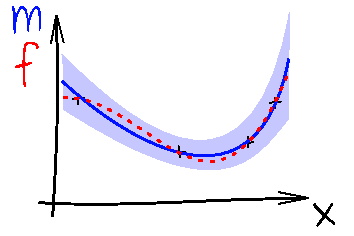
\includegraphics[height=5cm]{figures/ink_mconfint}
\end{center}
The confidence intervals can be used to obtain a \textbf{measure of uncertainty on the value of interest}.
\end{frame}

%%%%%%%%%%%%%%%%%%%%%%%%%%%%%%%%%%%%%%%%%%%%%%%%%%%%%%
\begin{frame}{}
In the sequel, we will use the following notations : 
\begin{itemize}
	\item The set of observation points will be represented by a $n \times d$ matrix $X=(X_1, ..., X_n)^t$
	\item The vector of observations will be denoted by $F$ : $F_i=f(X_i)$ (or $F=f(X)$).
\end{itemize}
We will now discuss two types of statistical models:
\begin{itemize}
	\item Linear regression
	\item Gaussian process regression
\end{itemize}
\end{frame}

%%%%%%%%%%%%%%%%%%%%%%%%%%%%%%%%%%%%%%%%%%%%%%%%%%%%%%
%%%%%%%%%%%%%%%%%%%%%%%%%%%%%%%%%%%%%%%%%%%%%%%%%%%%%%
\section{Linear Regression}
\subsection{}

%%%%%%%%%%%%%%%%%%%%%%%%%%%%%%%%%%%%%%%%%%%%%%%%%%%%%%
\begin{frame}{}
\begin{example}
	If we consider the following observations: 
\begin{center}
  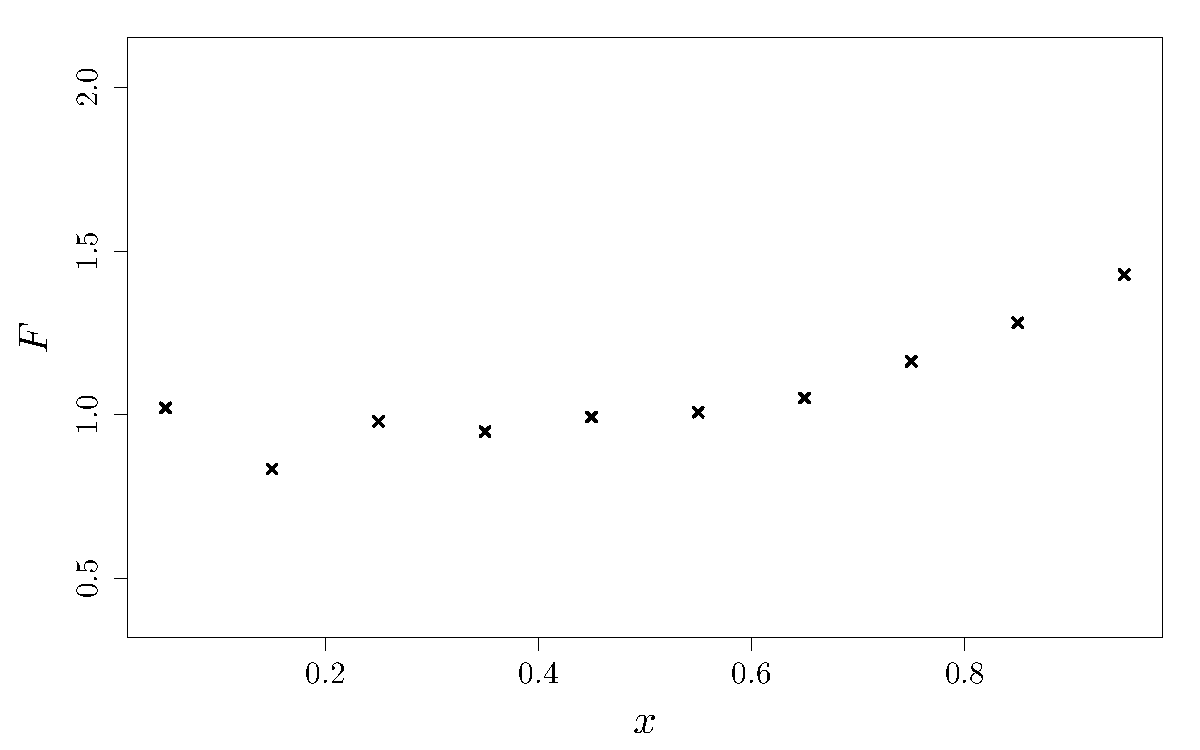
\includegraphics[height=5cm]{figures/R/linreg_0}
\end{center}
\vspace{-2mm}
\end{example}
\end{frame}

%%%%%%%%%%%%%%%%%%%%%%%%%%%%%%%%%%%%%%%%%%%%%%%%%%%%%%
\begin{frame}{}
\begin{example}
    We assume the observations are drawn from 
    $$ F_i = \sum_{k=0}^2 \beta_k b_k(X_i) + \varepsilon_i \qquad (= B(X_i) \beta  + \varepsilon_i )$$
	 with $b_0(x)=1,\ b_1(x)=x,\ b_2(x)=x^2$, unknown $\beta_i$ and i.i.d $\varepsilon_i$.
\begin{center}
  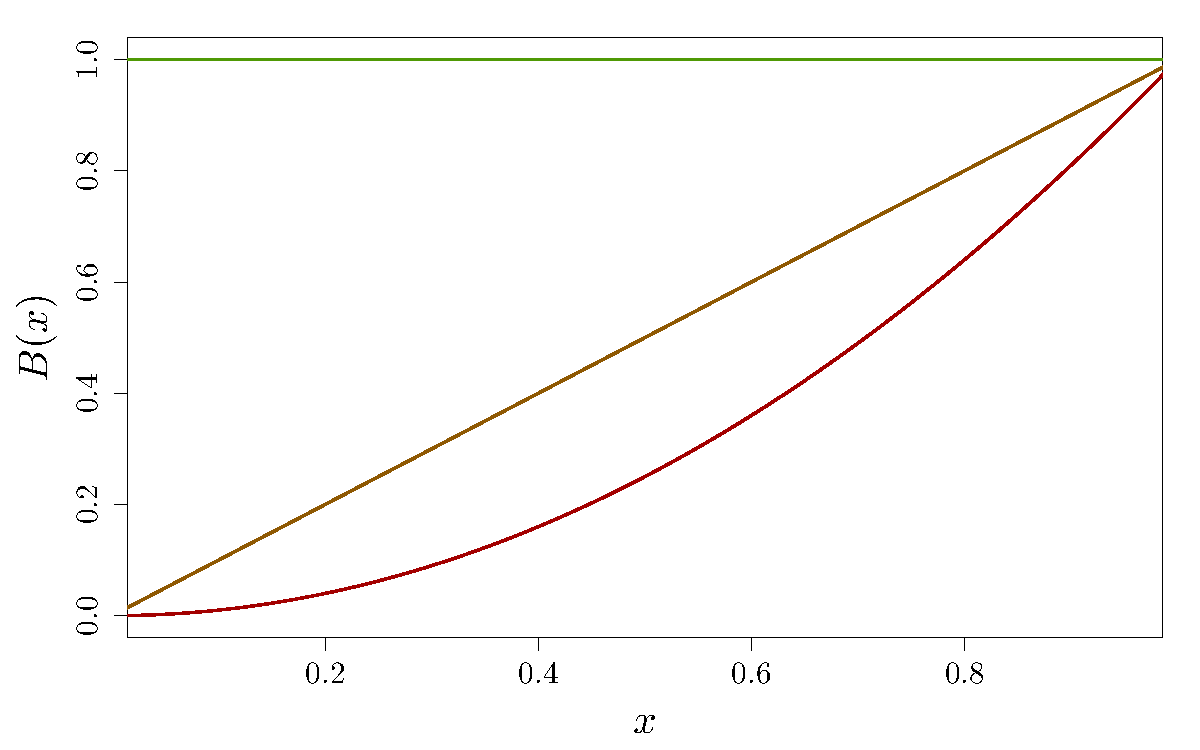
\includegraphics[height=4.9cm]{figures/R/linreg_1}
\end{center}
\end{example}
\end{frame}

%%%%%%%%%%%%%%%%%%%%%%%%%%%%%%%%%%%%%%%%%%%%%%%%%%%%%%
\begin{frame}{}
\begin{example}
The best linear unbiased estimator of $\beta$ is
$$\hat{\beta} = (B(X)^t B(X))^{-1} B(X)^t F.$$
We obtain $\hat{\beta} = (1.06,-0.61,1.04)^T$ and the model is:
\begin{center}
  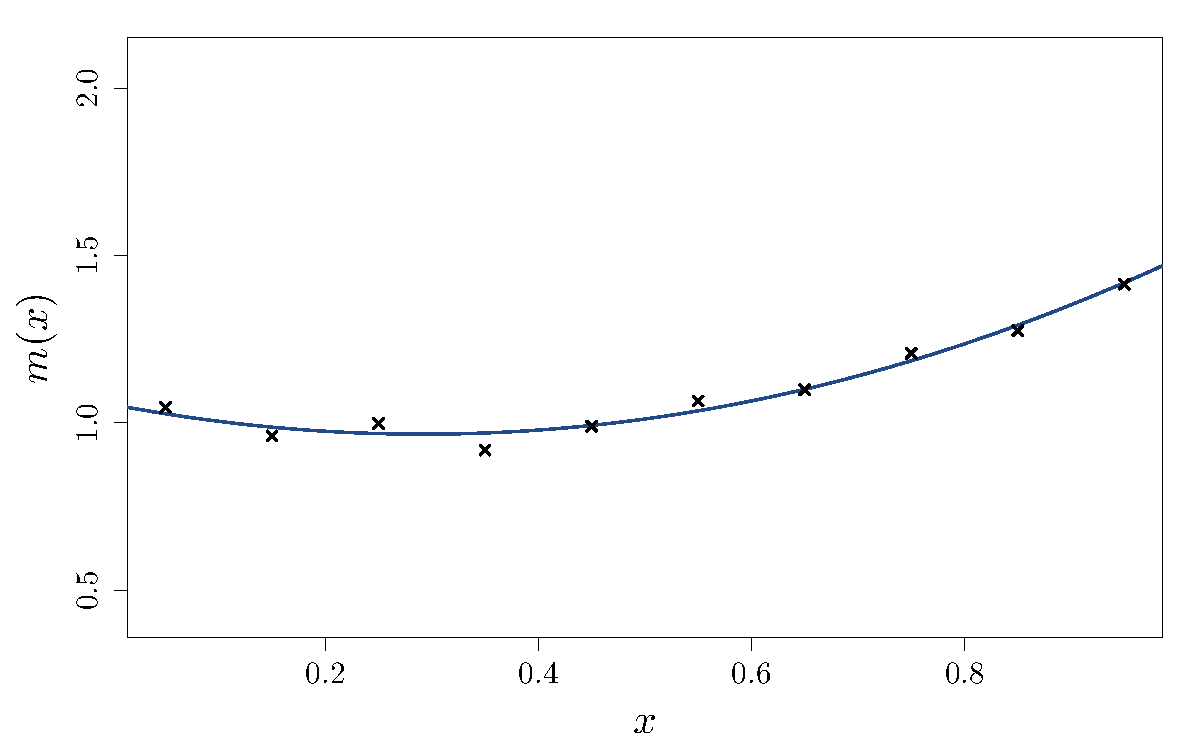
\includegraphics[height=5cm]{figures/R/linreg_2}
\end{center}
\end{example}
\end{frame}

%%%%%%%%%%%%%%%%%%%%%%%%%%%%%%%%%%%%%%%%%%%%%%%%%%%%%%
\begin{frame}{}
\begin{example}
There is of course an error between the true generative function and the model
\begin{center}
  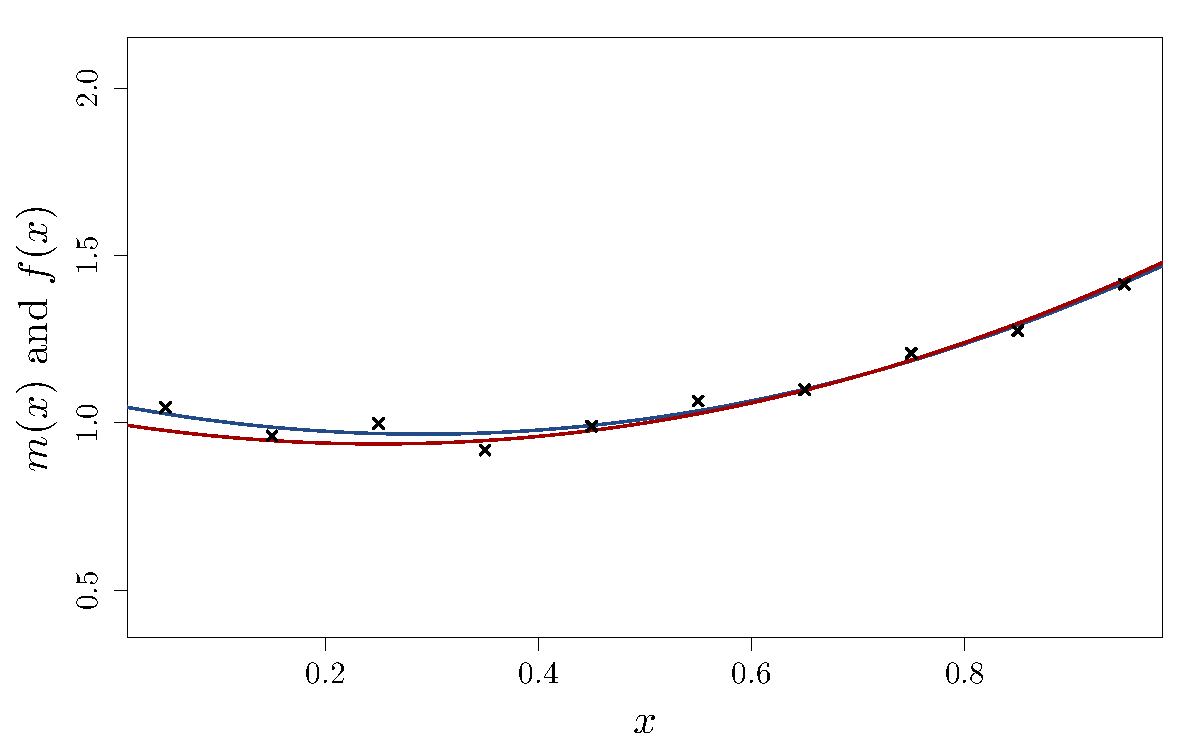
\includegraphics[height=5cm]{figures/R/linreg_3}
\end{center}
Can this error be quantified?
\end{example}
\end{frame}

%%%%%%%%%%%%%%%%%%%%%%%%%%%%%%%%%%%%%%%%%%%%%%%%%%%%%%
\begin{frame}{}
The initial assumption is $ F = B(X) \beta  + \varepsilon$ and we have computed an estimator of $\beta$:
$$\hat{\beta} = (B(X)^t B(X))^{-1} B(X)^t F.$$
$\hat{\beta}$ can thus be seen as a sample from the random variable:
$$\hat{\beta} = (B(X)^t B(X))^{-1} B(X)^t (B(X) \beta  + \varepsilon).$$ \\
\vspace{5mm}
What about the distribution of $\hat{\beta}$? \pause
\begin{itemize}
	\item Its expectation is $\beta$ \alert{$\Rightarrow$} The estimator is unbiased
	\item Its covariance matrix is $$(B(X)^t B(X))^{-1} B(X)^t \Cov[\varepsilon,\varepsilon^t] B(X) (B(X)^t B(X))^{-1}$$
	\item If $\varepsilon$ is multivariate normal, then $\hat{\beta}$ is also multivariate normal.
\end{itemize}
\end{frame}

%%%%%%%%%%%%%%%%%%%%%%%%%%%%%%%%%%%%%%%%%%%%%%%%%%%%%%
\begin{frame}{}
Sampling in the distribution of $\hat{\beta}$ gives us a large variety of models which represent the uncertainty about our estimation:
\begin{exampleblock}{Back to the example}
\begin{center}
  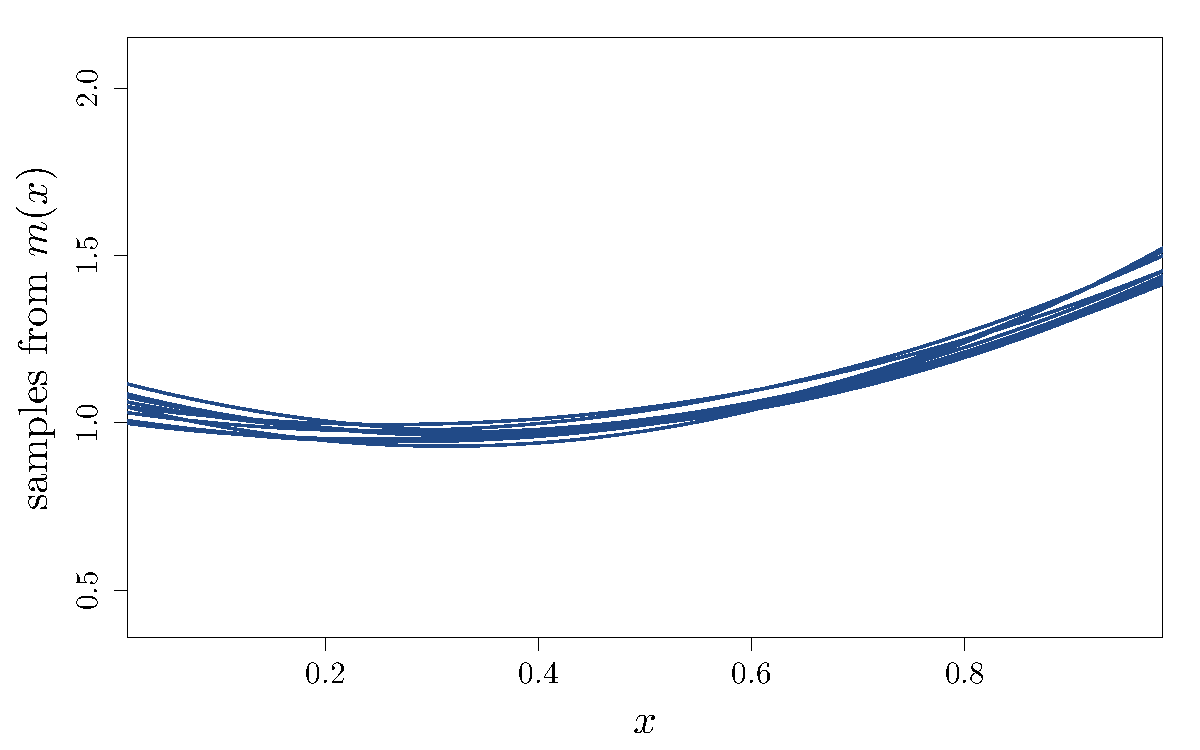
\includegraphics[height=5cm]{figures/R/linreg_4}
\end{center}
\end{exampleblock}
\end{frame}

%%%%%%%%%%%%%%%%%%%%%%%%%%%%%%%%%%%%%%%%%%%%%%%%%%%%%%
\begin{frame}{}
\begin{exampleblock}{Back to the example}
The previous picture can be summarized by showing the mean of $m$ and $95\%$ confidence intervals
\begin{center}
  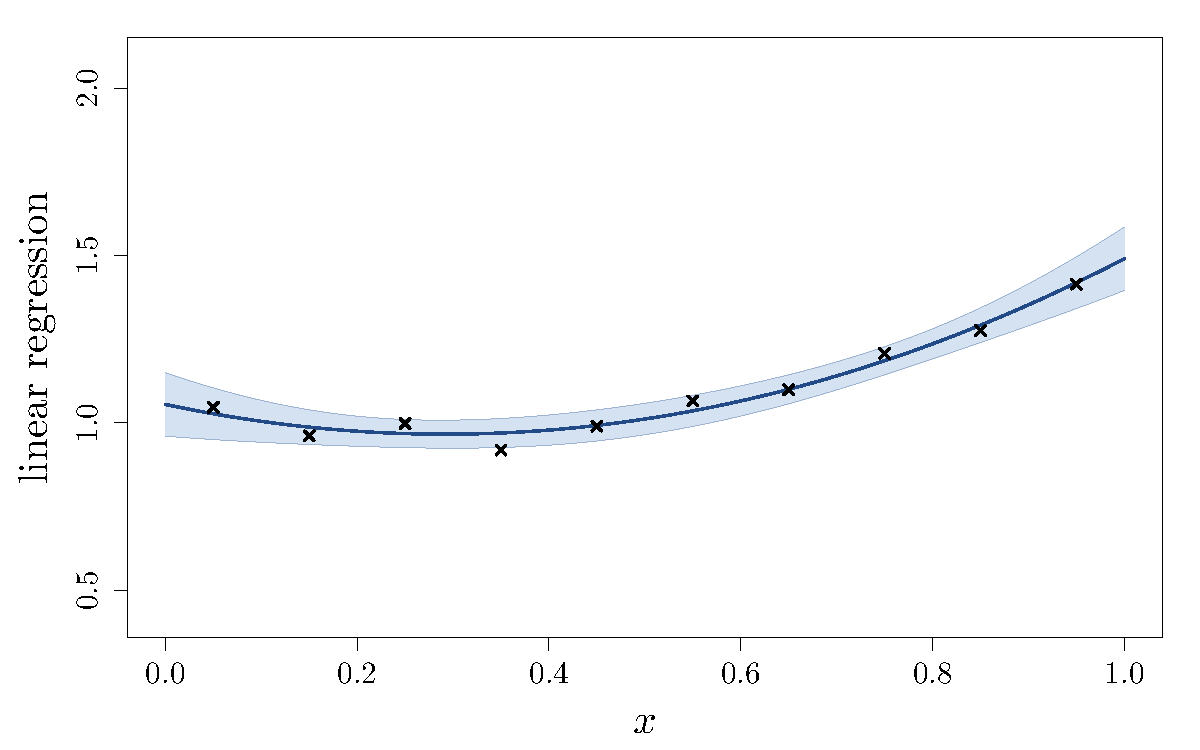
\includegraphics[height=5cm]{figures/R/linreg_5}
\end{center}
\end{exampleblock}
\end{frame}

%%%%%%%%%%%%%%%%%%%%%%%%%%%%%%%%%%%%%%%%%%%%%%%%%%%%%%
\begin{frame}{}
    This statistical model can be used for \textbf{uncertainty quantification}:
\begin{exampleblock}{Back to the example}
If we are interested in the value $x^\star$ minimizing $f(x)$:
\begin{center}
  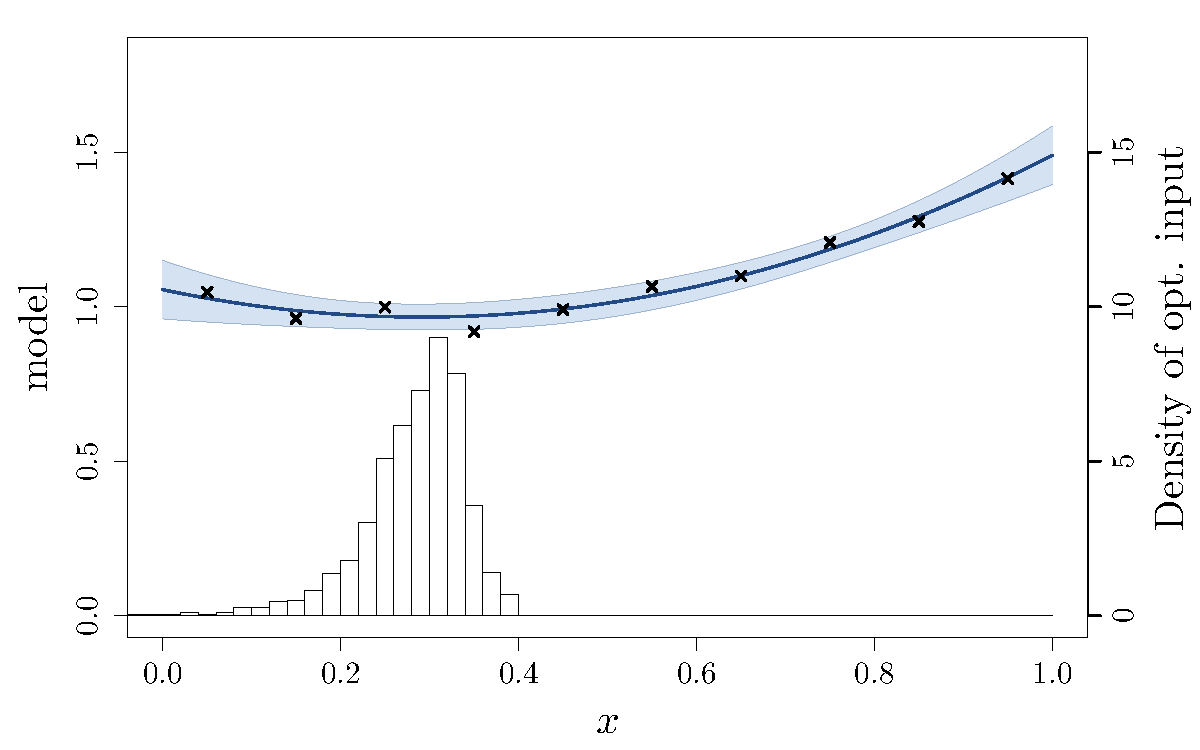
\includegraphics[height=5cm]{figures/R/linreg_6}
\end{center}
\end{exampleblock}
\alert{we obtain a distribution for $x^\star$.}
\end{frame}

%%%%%%%%%%%%%%%%%%%%%%%%%%%%%%%%%%%%%%%%%%%%%%%%%%%%%%
\begin{frame}{}
We could dedicate the entire course to linear regression models...
\begin{columns}[c]
\column{5cm}
\begin{itemize}
	\item model validation
	\item choice of basis functions
\end{itemize}
\column{6cm}
\begin{itemize}
	\item influence of input locations
	\item ...
\end{itemize}
\end{columns}
\vspace{10mm}
We will just stress a few \textbf{pros and cons of these models}:
\begin{itemize}
  \item[+] provide a good noise filtering
  \item[+] are easy to interpret
  \item[] \vspace{-5mm}
  \item[$-$] are not flexible (need to choose the basis functions)
  \item[$-$] do not interpolate
  \item[$-$] may explode when using high order polynomials (over-fitting)
\end{itemize}
\end{frame}

%%%%%%%%%%%%%%%%%%%%%%%%%%%%%%%%%%%%%%%%%%%%%%%%%%%%%%%%%%%%
\section{Conclusion}
\subsection{}

%%%%%%%%%%%%%%%%%%%%%%%%%%%%%%%%%%%%%%%%%%%%%%%%%%%%%%
\begin{frame}{}
\structure{Three things to remember:}\\ \vspace{3mm}
\begin{itemize}
	\item Statistical models are useful when little data is available. they allow to
	\begin{itemize}
		\item interpolate or approximate functions
		\item Compute quantities of interests (such as mean value, optimum, ...)
		\item Get an error measure
	\end{itemize}
	\item GPR is similar to linear regression but the assumption is much weaker (not a finite dimensional space)
	\item The GPR equations are
	\begin{equation*}
		\begin{split}
			m(x) & = k(x,X)k(X,X)^{-1}F\\
			c(x,y) &= k(x,y) - k(x,X)k(X,X)^{-1}k(X,y)
		\end{split}
	\end{equation*}
\end{itemize}
\end{frame}

%%%%%%%%%%%%%%%%%%%%%%%%%%%%%%%%%%%%%%%%%%%%%%%%%%%%%%
\begin{frame}{}
We still have many things to discuss about such models:
\begin{itemize}
	\item How to choose the observation points?
	\item How to validate the model?
	\item How to estimate the model (ie kernel) parameters?
\end{itemize}
This will be discussed during the next courses.\\
\vspace{10mm}
\structure{Reference}\\
Carl Edward Rasmussen and Chris Williams, \emph{Gaussian processes for machine learning}, MIT Press, 2006. (free version online).
\end{frame}


%%%%%%%%%%%%%%%%%%%%%%%%%%%%%%%%%%%%%%%%%%%%%%%%%%%%%%%%%%%%%%%%%%%%%%%%%%%%%%%
%%%%%%%%%%%%%%%%%%%%%%%%%%%%%%%%%%%%%%%%%%%%%%%%%%%%%%%%%%%%%%%%%%%%%%%%%%%%%%%
%%%%%%%%%%%%%%%%%%%%%%%%%%%%%%%%%%%%%%%%%%%%%%%%%%%%%%%%%%%%%%%%%%%%%%%%%%%%%%%
%%%%%%%%%%%%%%%%%%%%%%%%%%%%%%%%%%%%%%%%%%%%%%%%%%%%%%%%%%%%%%%%%%%%%%%%%%%%%%%
\end{document}













%%%%%%%%%%%%%%%%%%%%%%%%%%%%%%%%%%%%%%%%%%%%%%%%%%%%%%
%%%%%%%%%%%%%%%%%%%%%%%%%%%%%%%%%%%%%%%%%%%%%%%%%%%%%%
%%%%%%%%%%%%%%%%%%%%%%%%%%%%%%%%%%%%%%%%%%%%%%%%%%%%%%

\structure{}

\begin{center}
  \begin{tabular}{|c|cc|}

  \end{tabular}
\end{center}

###
%%%%%%%%%%%%%%%%%%%%%%%%%%%%%%%%%%%%%%%%%%%%%%%%%%%%%%
\begin{frame}{}

\end{frame}

###
\begin{block}{}

\end{block}

###
\begin{center}
\includegraphics[height=5cm]{figures/}
\end{center}

###
\begin{columns}[c]
\column{5cm}

\column{5cm}

\end{columns}
